\documentclass[10pt,a4paper,ngerman,oneside,]{article}
\newcommand\teamname{System.out.println(42);}
\newcommand\teammembers{Roland Haase\\ Thore Tiemann\\ Marcel Wienöbst}
\newcommand\university{Universität zu Lübeck}

\usepackage[log-declarations=false]{xparse}
\usepackage[utf8]{luainputenc}
\usepackage{luacode}
\usepackage[T1]{fontenc}
\usepackage{fontspec}
\usepackage[english]{babel}

\defaultfontfeatures{Ligatures=TeX}
\setmainfont{TeX Gyre Termes}
\setmonofont{Source Code Pro}

\usepackage[unicode,pdfencoding=auto,hidelinks]{hyperref}
\setlength{\columnseprule}{0.25pt}
\linespread{1.180}
\usepackage[left=1.5cm,right=.75cm,top=2.0cm,bottom=.8cm]{geometry}

\usepackage{fancyhdr}
\usepackage{lastpage}
\pagestyle{fancy}
\fancyhf{}
\fancyhead[R]{ACM ICPC Reference, page \bfseries\thepage/\pageref{LastPage}}
\fancyhead[L]{\university, Team: \teamname}

\usepackage{mathtools}
\usepackage{amsfonts}
\usepackage{amssymb}
\newcommand{\N}{\ensuremath{\mathbb{N}}}
\renewcommand{\C}{\ensuremath{\mathbb{C}}}
\newcommand{\lcm}{\ensuremath{\operatorname{lcm}}}
\newcommand{\bigo}[1]{\text{$\mathcal{O}\left(#1\right)$}}

\usepackage{algorithm}
\usepackage{algorithmic}

\usepackage{graphicx}
\usepackage{pdfpages}
\usepackage{xcolor}
\definecolor{darkgreen}{rgb}{0,0.5,0}
\definecolor{uni}{RGB}{0,75,90}

\usepackage{listings}
\lstset{numbers=left,
        captionpos=b,
        emptylines=*1,
        language=Java,
        numberstyle=\ttfamily\tiny,
        basicstyle=\ttfamily\footnotesize,
        identifierstyle=\color{black},
        keywordstyle=\ttfamily\bfseries\color{uni},
        commentstyle=\color{darkgreen},
        stringstyle=\color{violet},
        backgroundcolor=\color{black!5},
        frame=lines,
        framerule=1.0pt,
        showspaces=false,
        showtabs=false,
        tabsize=2,
        numbersep=5pt,
        mathescape=true,
        breaklines=true,
        % breakatwhitespace=true,
        % prebreak=\raisebox{0ex}[0ex][0ex]{\ensuremath{\space\color{red}\rhookswarrow}},
        % postbreak=\raisebox{0ex}[0ex][0ex]{\ensuremath{\color{red}\hookrightarrow\space}}
}
\usepackage{multicol}
\setlength{\parindent}{0pt}

\newenvironment{algo}{%
    % variables
    \def\algorithmName{\color{red}Title not set}%
    \def\algorithmDescription{\color{red}Description not set}%
    \def\algorithmFile{No File given}%
    \def\algorithmComplexity{?}%
    \def\algorithmHash{-}%
    % setter
    \newcommand{\setAlgorithmName}[1]{\def\algorithmName{##1}}%
    \newcommand{\setAlgorithmDescription}[1]{\def\algorithmDescription{##1}}%
    \newcommand{\setAlgorithmFile}[1]{\def\algorithmFile{##1}}%
    \newcommand{\setAlgorithmComplexity}[1]{\def\algorithmComplexity{##1}}%
    \newcommand{\setAlgorithmHash}[1]{\def\algorithmHash{##1}}%
}{%
    \subsection{\algorithmName}%
    \algorithmDescription%
    \lstinputlisting[title=
    {\footnotesize{\textbf{MD5:}\;\texttt{\algorithmHash}\;\mid\;%
    $\mathcal{O}(\algorithmComplexity)$}}]{\algorithmFile}%
}%

\title{Team Contest Reference}
\author{\university}

\begin{document}
\vspace{-5mm}
\begin{center}
	\begin{minipage}{0.3\textwidth}
	  
\includegraphics[scale=.8,clip,trim=.4cm 0cm 6.4cm 0cm,scale=0.89]{img/logo_uzl.pdf}
    \end{minipage}
	\begin{minipage}{0.35\textwidth}
      \begin{center}
	    \LARGE{\bfseries Team Contest Reference}\\
        \textbf{Team:} {\teamname}
      \end{center}
    \end{minipage}
	\begin{minipage}{0.3\textwidth}
      \flushright
      \itshape\teammembers
    \end{minipage}
\end{center}
\thispagestyle{fancy}
\tableofcontents

\begin{multicols}{2}
% \vfill
\vspace{1em}{\centering
\hfill\begin{tabular}{rl}
	\hline $n$ & Runtime $100\cdot 10^{6}$ in $3$s \\\hline
	$[10,11]$ & $\mathcal{O}(n!)$ \\
	$<22$ & $\mathcal{O}(n2^n)$ \\
	$\leq 100$ & $\mathcal{O}(n^4)$ \\
	$\leq 400$ & $\mathcal{O}(n^3)$ \\
	$\leq 2.000$ & $\mathcal{O}(n^2\log n)$ \\
	$\leq 10.000$ & $\mathcal{O}(n^2)$ \\
	$\leq 1.000.000$ & $\mathcal{O}(n\log n)$ \\
	$\leq 100.000.000$ & $\mathcal{O}(n)$ \\\hline
\end{tabular}\hfill}

\vspace{1em}
\noindent
\texttt{byte} (8 Bit, signed): -128 \dots 127\\
\texttt{short} (16 Bit, signed): -32.768 \dots 23.767\\
\texttt{integer} (32 Bit, signed): -2.147.483.648 \dots 2.147.483.647\\
\texttt{long} (64 Bit, signed): $-2^{63}$\dots $2^{63}-1$\\

\newcommand{\hash}[1]{{\bfseries MD5:} ~\texttt{#1}}
\vspace{1.2em}\noindent {\textbf{MD5:}} \texttt{\small cat <string>| tr -d [:space:] | md5sum}\\

\newpage
% \begin{multicols}{2}
\luadirect{ require('parseCode.lua') }
\luadirect{ removeTmpFiles() }
\luadirect{ parse() }
\luadirect{ removeTmpFiles() }
\newpage
\end{multicols}

\section{Java Knowhow}
\subsection{System.out.printf() und String.format()}
\textbf{Syntax}: \texttt{\%[flags][width][.precision][conv]}

\textbf{flags}: \\ \begin{tabular}{ll}
  \texttt{-} & left-justify (default: right) \\
  \texttt{+} & always output number sign \\
  \texttt{0} & zero-pad numbers \\
  (space)    & space instead of minus for pos. numbers \\
  \texttt{,} & group triplets of digits with ,
\end{tabular}

\textbf{width} specifies output width

\textbf{precision} is for floating point precision

\textbf{conv}: \\ \begin{tabular}{ll}
  d & byte, short, int, long \\
  f & float, double \\
  c & char (use C for uppercase) \\
  s & String (use S for all uppercase)
\end{tabular}

\subsection{Speed up IO}
Use \texttt{BufferedReader br = new BufferedReader(new
InputStreamReader(System.in));}

Use \texttt{Double.parseDouble(Scanner.next())}



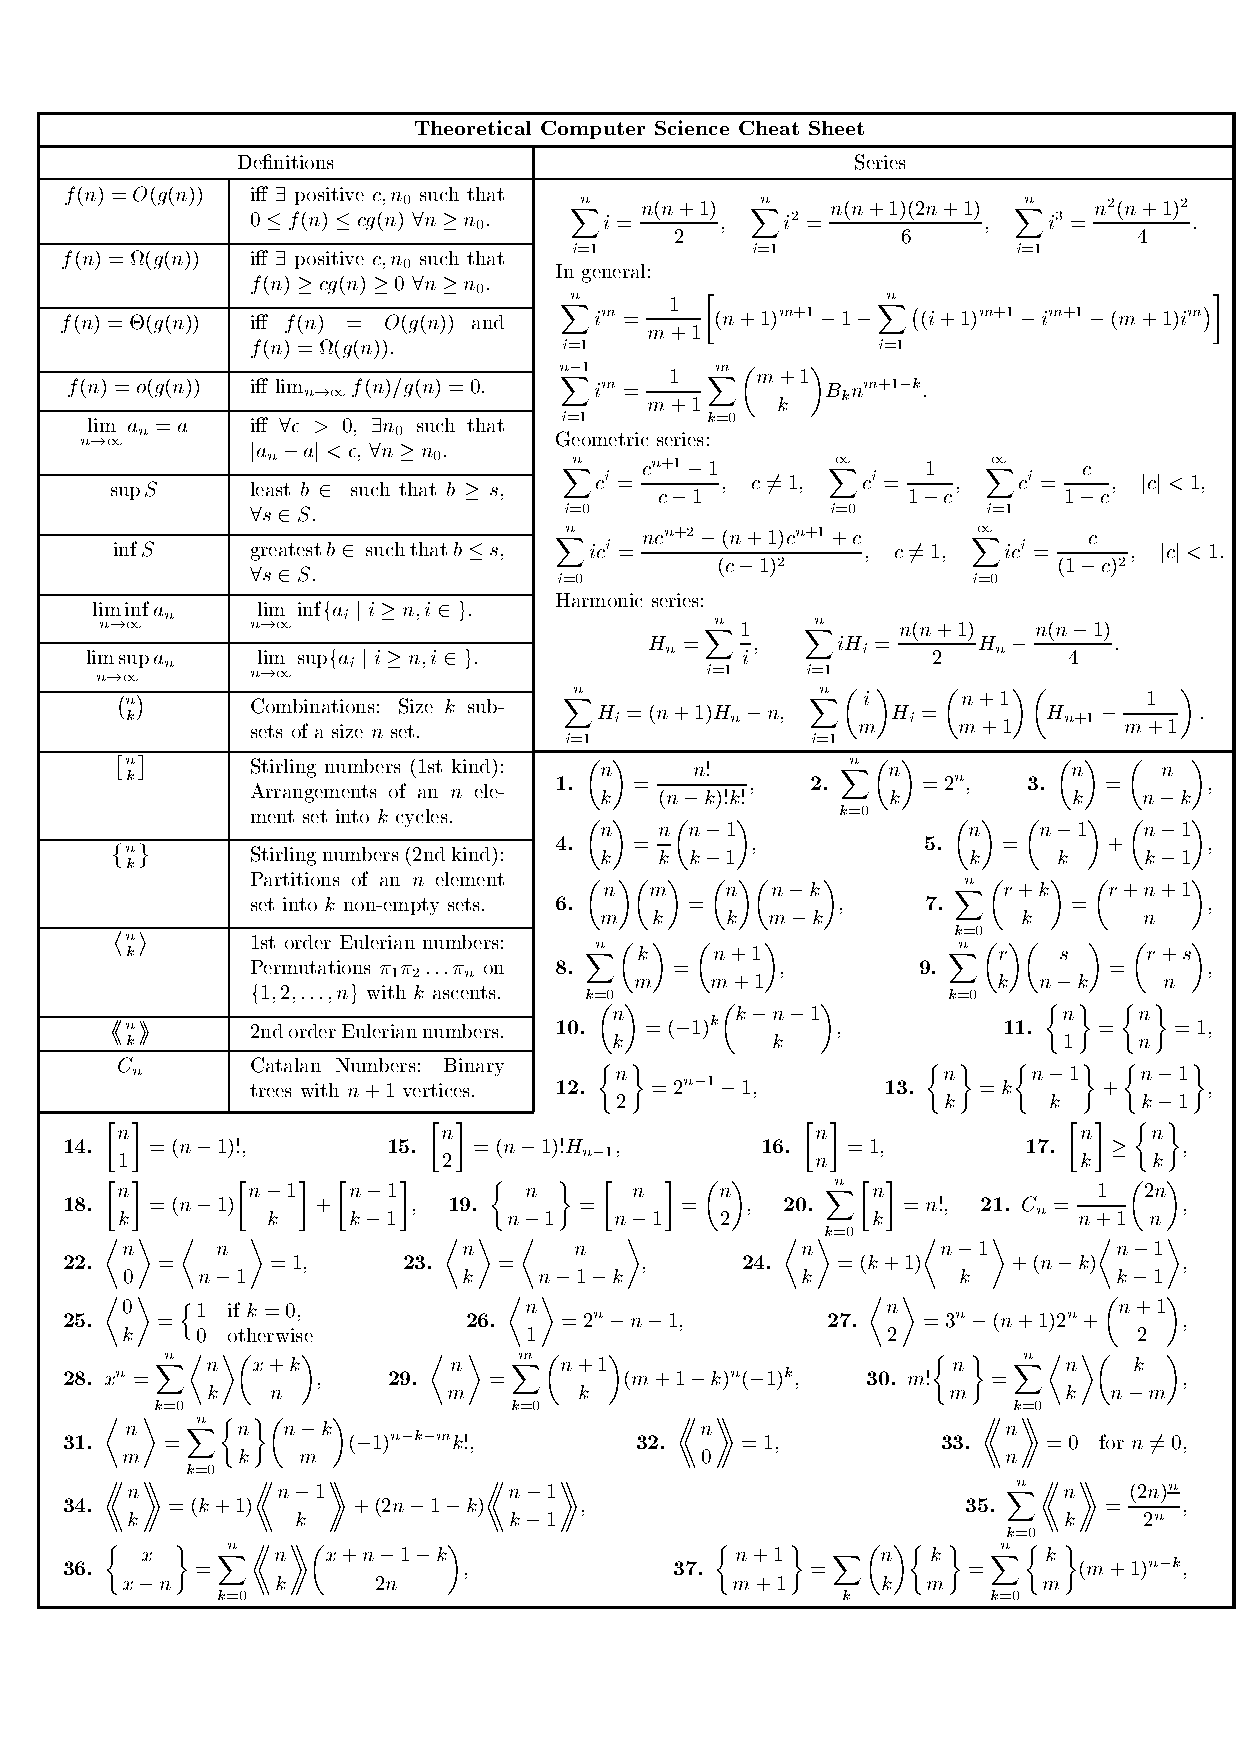
\includepdf[pages=-,clip,trim=5mm 17mm 0mm 17mm,scale=0.95,pagecommand={\pagestyle{plain}}]{tcs-cheat-sheet.pdf}

\end{document}
